\subsection{谱误差与目标反馈在常用深度上汇合}
Error-NS在主对照的30次选择中都选了NS5。Probe-NS选了28次NS5和2次NS3，
终点验证损失为4.8150，固定NS5为4.8118。
两个策略在训练中频繁遇到相同的最佳候选，这与冻结模型在实际步长下的排序结果一致。

三条阶段匹配重放与对应的反馈序列逐项相同。
种子0一直使用NS5。种子1和2在第900步改用NS3，在最终一步切回NS5。
最后一段中两种深度的驻留长度分别为100步和1步，保持实际更新频率便保留了它们的位置。
附录表\ref{tab:v2replay}给出每条序列和实际改动步数。

补充重放把种子1和2的100步NS3区间从第900步移到第800步。
两条轨迹各有200次更新改变深度，深度频率与探测计算保持相同。
相对当次反馈，提前后的测试损失分别降低0.00590和0.00581 nats/token。
两条提前重放与同种子固定NS5的测试损失差分别为$+0.00009$和$-0.00014$。
移动这一个区间后，测试损失回到固定NS5的水平。


\subsection{扩大规模、延长训练与改变更新尺度}
在51.1M参数模型中，隐藏矩阵参数增至25.17M。
固定NS5将WikiText103的终点验证损失从匹配AdamW的5.0354降至4.6493，
Probe-NS取得4.6506。该规模下的30次反馈选择有26次落在NS5。

在小模型的幅度消融中，固定AdamW学习率后，RMS-Adam取得5.1398，
标准AdamW为5.1240。固定NS5学习率后，Moonlight更新尺度取得4.8007，
逐矩阵匹配RMS为4.8118。两组消融直接测量了幅度变换对各自更新规则的影响。

TinyStories采用独立筛选的矩阵学习率。在26.5M参数模型上，AdamW、固定NS5和Probe-NS的终点验证损失
分别为2.5396、2.3466和2.3499 nats/token。Probe-NS的30次选择中有26次采用NS5。

长程WikiText103组分别筛选NS3和NS5，选出的峰值学习率均为0.003。
训练处理2048万token后，NS3和NS5的终点验证损失分别为4.3659和4.2648。
三个种子中，NS3与NS5的验证损失差为0.0994至0.1024 nats/token，平均测试损失差为0.1028。

三个语料与规模设置共有九对固定NS5和Probe-NS的测试结果。
固定NS5在其中八对的损失更低，一对相同。三组的平均差介于0.0034与0.0046 nats/token。


\begin{table}[htbp]\centering\small
\caption{模型规模、语料和训练长度的对照。各方法使用三个配对种子，损失单位为nats/token。}
\label{tab:v2transfer}
\begin{tabular}{llrr}
\toprule
实验设置 & 方法 & 终点验证损失 & 测试损失 \\ \midrule
WikiText103，51.1M & AdamW & $5.0354\pm0.0039$ & $5.0422\pm0.0050$ \\
 & NS5 & $4.6493\pm0.0034$ & $4.6559\pm0.0024$ \\
 & Probe-NS & $4.6506\pm0.0037$ & $4.6606\pm0.0059$ \\
\addlinespace
TinyStories，26.5M & AdamW & $2.5396\pm0.0100$ & $2.4994\pm0.0107$ \\
 & NS5 & $2.3466\pm0.0009$ & $2.3094\pm0.0012$ \\
 & Probe-NS & $2.3499\pm0.0025$ & $2.3128\pm0.0041$ \\
\addlinespace
WikiText103，20.48M token & NS3 & $4.3659\pm0.0029$ & $4.3563\pm0.0058$ \\
 & NS5 & $4.2648\pm0.0014$ & $4.2536\pm0.0022$ \\
\bottomrule
\end{tabular}

\end{table}

\begin{figure}[htbp]\centering
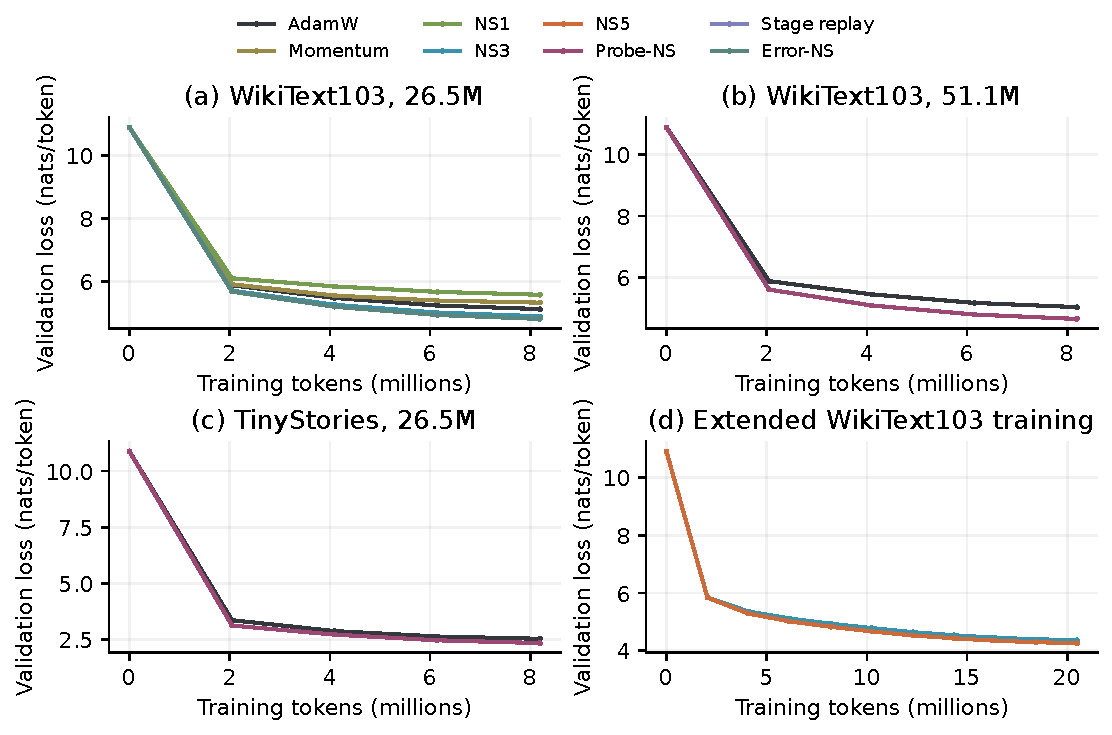
\includegraphics[width=\linewidth]{figures_v2/v2_training.pdf}
\caption{完整语言训练中的验证损失。各点为三个种子的均值，阴影为一个样本标准差。}
\label{fig:v2train}
\end{figure}

\subsection{正交化与深度选择的计算开销}
在共同输入的同步计时中，26.5M模型的NS3和NS5优化器耗时中位数分别为52.65和62.35\,ms。
在51.1M模型中，这两个数值增至112.72和135.16\,ms。
图\ref{fig:v2profile}分解了固定深度及对照方法的每步耗时。

Probe-NS在选择步同时生成三个候选并计算其批次损失。两个模型的选择步优化器耗时中位数
分别为292.60和480.35\,ms。按每100步选择一次计算，相对固定NS5，选择开销折合每步增加2.30和3.45\,ms。
Error-NS在选择步以SVD计算参考极因子，小模型和大模型的相应耗时为1.95和9.02\,s。
这组计时将更新深度的运算代价和当次选择依据的运算代价分开。

\begin{figure}[htbp]\centering
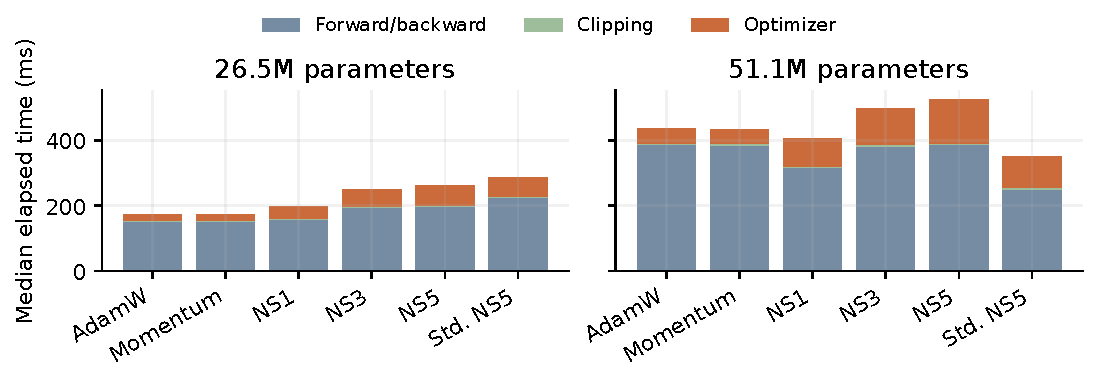
\includegraphics[width=\linewidth]{figures_v2/v2_profile.pdf}
\caption{同一模型规格下的同步计时。前向与反向、梯度裁剪和优化器分别取12次测量的中位数。}
\label{fig:v2profile}
\end{figure}

